   \documentclass[12pt]{article}

% sbc template
\usepackage{sbc-template}
\usepackage{graphicx,url}
\usepackage[utf8]{inputenc}

% equations
\usepackage{mathtools}
\usepackage{multicol}
\usepackage[version=4]{mhchem}
\usepackage{multicol}

% code snippets
\usepackage{graphicx}
\usepackage{listings}
\usepackage{xcolor}

% roman enums
\usepackage{enumitem}

% remove listing name
\renewcommand{\lstlistingname}{}

% gro language definition
\definecolor{COLOR_COMMENTS}{RGB}{16, 97, 35}
\definecolor{COLOR_BACKGROUND}{RGB}{230, 230, 230}
\lstdefinelanguage{GROLANG}{
  morekeywords    =   {include,program,rate,ecoli},
  sensitive       =   false,
  morecomment     =   [l]{//},
  morestring      =   [b]",
}
\lstdefinestyle{GROSRC}
{
  language          =   GROLANG,
  basicstyle        =   \scriptsize\ttfamily,
  keywordstyle      =   \color{black}\bfseries,
  extendedchars     =   true,
  commentstyle      =   \color{COLOR_COMMENTS},
  backgroundcolor   =   \color{COLOR_BACKGROUND},
  frame             =   single,
  tabsize           =   4,
  breaklines        =   true,
  showstringspaces  =   false,
}

% parsed.intermediate style definition
\lstdefinestyle{INTERMEDIATE}{
  basicstyle        =   \scriptsize\ttfamily,
  backgroundcolor   =   \color{COLOR_BACKGROUND},
  otherkeywords     =   {compartment, var, const, in},
  keywordstyle      =   \color{black}\bfseries,
  frame             =   single,
  tabsize           =   4,
  caption           =   Compiled dummy.,
  breaklines        =   true,
  showstringspaces  =   false,
}

% sbml style definition
\lstdefinestyle{SBML}
{
  basicstyle        =   \scriptsize\ttfamily,
  keywordstyle      =   \color{black}\bfseries,
  otherkeywords     =   {reactionlist, reaction, species, <, >, /, listOfSpecies, listOfCompartments, compartment, sbml, xmlns, version, parameter, listOfParameter, reaction, listOfReactions, listOfReactants, specieReference, listOfProducts, kineticLaw, model, math, ?xml},
  extendedchars     =   true,
  commentstyle      =   \color{COLOR_COMMENTS},
  backgroundcolor   =   \color{COLOR_BACKGROUND},
  frame             =   single,
  tabsize           =   4,
  breaklines        =   true,
  showstringspaces  =   false,
}

% contribution1 = Facilitating the synthesis process of biological devices through higher level language abstractions.
%contribution2 = propose an compilation scheme for any higher level language to SBML based on the construction of a parsing and translating tool.

% begin paper
\sloppy
\title{A compilation scheme to provide high level language abstractions to the synthesis process of biological devices}
\author{Alek Frohlich\inst{1}, Gustavo Biage\inst{1}}
\address{Departamento de Informatica e Estatística – Universidade Federal de Santa Catarina \\
Florianopolis – SC – Brazil
  \email{\{alek.frohlich,gustavo.c.biage\}@grad.ufsc.br}
}
\begin{document}
\maketitle
\begin{abstract}


    The growth of research areas such as synthetic biology and systems biology leads to an increased tendency to develop larger mathematical models for describing complex biological behavior. In order for those models to be implementable in living systems, scientists must have access to a synthesis process of biological devices that is robust and automated. This process ought to provide higher levels of abstraction than the ones found by tinkering with low level components such as promoters and transcription factors. The present work aids the development of such processes by translating a subset of the gro programming language into SMBL documents, and thus speeding up the synthesis process due to facilitating the design of biological devices through the use of a higher level language.


\end{abstract}
\section{Introduction}


    The development of an automated synthesis process is essential to the scalability of synthetic biological devices. Without it, each device has to be designed individually, leading to an error-prone process not well suited for the development of large devices. Many substitutes to this primitive procedure have been proposed, one of them, the Cello framework, automates genetic circuit design with the assistance of a genetic component library. The framework searches the component library for parts compliant with the specifications of the Verilog code to produce an equivalent implementable genetic circuit that is also minimum cost \cite{Nielsenaac7341}. 
    
    Cello was heavily inspired by the synthesis process of semi-conductor based electronics. The inspiration is made clearer by the choice of Verilog as the framework's interface. Such an approach may not be ideal as there clearly isn't a one to one correspondence between both processes. An alternative would be to model the high level behavior of biological devices through a language capable of accounting for their unique aspects, e.g. the uncertainty associated with it's reactions occurrence\footnote{The concentration and distribution of molecules dictate the whether biochemical reactions occur}.
    
    Systems Biology Markup Language (SBML) is a useful language for describing biochemical models of synthetic and systems biology \cite{Hucka2003}. Although not being able to fully represent the aforementioned aspects of biological devices, SBML does manage express them in more natural terms. However, one may question it's expressiveness as a programming language considering that even small models can be cumbersome to write. The present work proposes a solution that circumvents SBML's lack of high level abstractions, enabling it to be used as the entry point to the physical implementation stage of a synthesis process. The solution consists in abstracting many of SBML's core language features in favor of higher level constructs found in the gro programming.
    
    Gro is a language for programming, modeling, specifying and simulating the behavior of cells in growing microcolonies of microorganisms. Gro models are comprised of global variables, program declarations and bacterial instantiations. Programs behave similarly to functions in imperative programming languages. They are used to describe a functionality that will be executed at every time step of the simulation. Inside such construct, there may appear variable definitions and guarded code blocks. Guarded blocks are blocks of code that only execute in case the Boolean expression guarding them evaluates to true. A bacteria can be instantiated with any amount of said programs \cite{Jang2012}.
    
    The language parser works in conjunction with a framework called Tellurium. Tellurium is a Python-based modeling environment for systems and synthetic biology \cite{Choi2018}. The language parser verifies the correctness of the gro source code. Valid programs are translated to an intermediate format which, in turn, becomes the final SBML document through the assistance of Tellurium.

    The rest of the paper is structured as follows: Section 2 introduces the language parser and explain the process of converting gro files to SBML models from start to finish. Section 3 presents a case study on the application of the proposed language parser along with an evaluation of its abstractions, and Section 4 presents our final considerations and future works.


\section{Code Generation}\label{sec:code-gen}


    In this section we describe gro's compilation process (depicted at Figure~\ref{fig:compilation_steps}): First, the gro source code is validated, that is, it’s checked against syntax errors, such as missing semicolon in rate statements and semantic error such as using undeclared variables; Then the code gets translated to an intermediate representation called Antimony \cite{Smith2009}; Finally, Tellurium uses libSBML and libAntimony to convert the given Antimony file down to an SBML document.
    
    \begin{figure}[h]
        \centering
        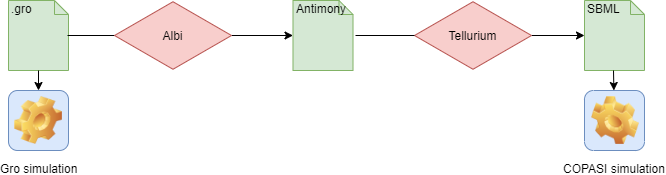
\includegraphics[scale = 0.6]{architecture.png}
        \caption{Flow chart of the compilation steps.}
        \label{fig:compilation_steps}
    \end{figure}


\subsection{Parsing}

    As mentioned before, the code submitted to the compiling process is parsed and translated to an intermediate language called Antimony, a modular model definition language \cite{Smith2009}. The proposed parser recognizes a subset of gro's syntax. The subset is composed of global variable declarations, program definitions and E. coli instantiations. Parameters, messages and guarded statements are also recognized, however no semantic value is assigned to them given that control statements and user interaction do not fit the context of an SBML model. The following is an example of gro code containing the syntactical constructs just described.

    \begin{lstlisting}[style=GROSRC, caption=Example gro code.]
 include gro

 program prog() := {
     E := 25;
     F := 75 + E;
     K := 2 + F + E;
     rate(K) : { E := E + 1, F := F - 1 };
 };

 program dupl(X) := {
     E := 25 + X;
     F := 75 + E;
     K := 2 + F + E;
     rate(K*40) : { E := E + 1, F := F - 1 };
 };

 ecoli([], program prog() + dupl(10));
 ecoli([], program prog());
\end{lstlisting}

\subsection{Translating}
    
    After the parsing, the code is translated to Antimony. The resultant file will be further submitted to Tellurium. Gro code translation into Antimony occurs as follows:


    \begin{enumerate}[label=(\roman*)]
        \item Gro files are represented as an Antimony file.
        \item E. coli instantiated in the gro source are declared as compartments.
        \item Rate statements are represented as \ce{$s_{1}$ R_{1} + $s_{2}$ R_{2} + ... + $s_{n}$ R_{n} -> $t_{1}$ P_{1} + $t_{2}$ P_{2} + ... + $t_{n}$ P_{n}}. Where the stoichiometric constants $s_{i}$ and $t_{j}$ denote the number of times the variables  $R_{i}$ and $P_{j}$ were decremented/incremented inside the guarded block.
        \item Variables that do not appear in such reactions are considered global constants.
        \item Code blocks guarded by gro's rate function appear next to their reactions.
    \end{enumerate}
    
    Also, symbols declared inside program definitions are renamed to avoid name space clashes between multiple programs instantiated in the same compartment.
    
\subsection{Compiling}

    As mentioned before, after translation the code is submitted to Tellurium to generate the final SBML document. Listing 2 shows a cleaned version of the generated SBML where some reactions and SBML syntax has been omitted to avoid cluttering\footnote{The reaction shown bellow is the one from \textit{prog}, instantiated in the first E. coli. Other tags not shown include the preamble declaration of the XML and the SBML document.}. The gro to SBML mapping is presented bellow:
    
    \begin{enumerate}[label=(\roman*)]
        \item Gro files are represented as models.
        \item E. coli are represented as compartments.
        \item Variables are identified as species when participating in a reaction, otherwise they are marked as constant and identified as parameters.
        \item Reactions are marked irreversible\footnote{Gro reactions are marked irreversible since it does not support reversible ones.} and have their lists of reactants and products filled based on what variables are being decremented and incremented, respectively.
        \item Expressions inside rate functions that guard blocks of code become kinetic law constants inside reactions.
    \end{enumerate}
    

    \begin{lstlisting}[style=SBML, caption=Generated SBML document.]
  <model metaid="__main" id="__main">
    <listOfCompartments>
      <compartment id="ECOLI0" spatialDimensions="3" size="1" constant="true"/>
      <compartment id="ECOLI1" spatialDimensions="3" size="1" constant="true"/>
    </listOfCompartments>
    <listOfSpecies>
      <species id="ECOLI0_prog_E" compartment="ECOLI0" initialConcentration="25" constant="false"/>
      <species id="ECOLI0_prog_F" compartment="ECOLI0" initialConcentration="100" constant="false"/>
      <species id="ECOLI0_dupl_E" compartment="ECOLI0" initialConcentration="35" constant="false"/>
      <species id="ECOLI0_dupl_F" compartment="ECOLI0" initialConcentration="110" constant="false"/>
      <species id="ECOLI1_prog_E" compartment="ECOLI1" initialConcentration="25" constant="false"/>
      <species id="ECOLI1_prog_F" compartment="ECOLI1" initialConcentration="100" constant="false"/>
    </listOfSpecies>
    <listOfParameters>
      <parameter id="ECOLI0_prog_K" value="127" constant="true"/>
      <parameter id="ECOLI0_dupl_K" value="147" constant="true"/>
      <parameter id="ECOLI1_prog_K" value="127" constant="true"/>
    </listOfParameters>
    <listOfReactions>
      <reaction id="_J0" reversible="true" fast="false">
        <listOfReactants>
          <speciesReference species="ECOLI0_prog_F" stoichiometry="1" constant="true"/>
        </listOfReactants>
        <listOfProducts>
          <speciesReference species="ECOLI0_prog_E" stoichiometry="1" constant="true"/>
        </listOfProducts>
        <kineticLaw>
          <math xmlns="http://www.w3.org/1998/Math/MathML">
            <ci> ECOLI0_prog_K </ci>
          </math>
        </kineticLaw>
      </reaction>
      ...
    </listOfReactions>
  </model>
\end{lstlisting}


\section{Case Study: The Repressilator}


    This section presents the experiment used to evaluate the proposed compilation process. The experiment consists on executing the Repressilator (a well-known biological device) in gro's built-in simulator and comparing the Octave output to the simulation of the SBML document obtained by compiling the code according to the process described at Section \ref{sec:code-gen}. The SBML simulations were done through Copasi, a pathway simulator \cite{Hoops2006}.
    

\subsection{Repressilator Model}

    \begin{figure}[ht]
        \centering
        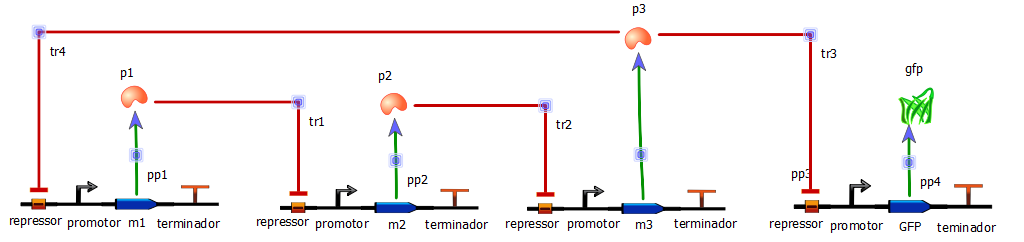
\includegraphics[scale = 0.45]{repressilator_model.png}
        \caption{Repressilator's genetic regulatory network.}
        \label{fig:repressilator_model}
    \end{figure}
    
    The Repressilator is a genetic regulatory network constituted by stitching together promoter-repressor pairs. It was first conceptualized by \cite{Elowitz2000}, who used the genes LacI and letR from E. coli and cI from phage lambda to build a three-repressor scheme. As illustrated in Figure~\ref{fig:repressilator_model}, the Repressilator works based on the fact that each gene expresses a protein which represses the next gene in the loop, meaning that a constituent gene in high concentration represses itself indirectly, leading to oscillatory behavior. In the original experiment, there was another biological component involved: the reporter, a green fluorescent protein (GFP) producing gene. It was used to visualize the network's oscillation.
    
\subsection{Mathematical Model}\label{math-model}
    
    As shown in \cite{Elowitz2000}, the high-level model from Figure~\ref{fig:repressilator_model} could also be presented as the following system of Ordinary Differential Equations (ODE).
    
    \begin{equation}
    \begin{aligned}[c]
        \frac{dm_{1}(t)}{dt} & = \alpha_{0} + \frac{\alpha}{1 + p_{3}(t)^{n}} - m_{1}(t) & \\
        \frac{dm_{2}(t)}{dt} & = \alpha_{0} + \frac{\alpha}{1 + p_{1}(t)^{n}} - m_{2}(t) & \\
        \frac{dm_{3}(t)}{dt} & = \alpha_{0} + \frac{\alpha}{1 + p_{2}(t)^{n}} - m_{3}(t) &
    \end{aligned}
    \begin{aligned}[c]
        \frac{dp_{1}(t)}{dt} & = \beta \cdot m_{1}(t) - \beta \cdot p_{1}(t) \\
        \frac{dp_{2}(t)}{dt} & = \beta \cdot m_{2}(t) - \beta \cdot p_{2}(t) \\
        \frac{dp_{3}(t)}{dt} & = \beta \cdot m_{3}(t) - \beta \cdot p_{3}(t)
    \end{aligned}
    \end{equation}

\subsection{Gro Code}

    The gro code for the Repressilator is presented below.
    
    \begin{lstlisting}[style=GROSRC]
 rate(alfa0) : { m1 := m1 + 1, m2 := m2 + 1, m3 := m3 + 1 };
 rate(alfa / (1 + p3^n)) : {m1 := m1 + 1};
 rate(m1) : {m1 := m1 - 1};
 rate(alfa / (1 + p1^n)) : {m2 := m2 + 1};
 rate(m2) : {m2 := m2 - 1};
 rate(alfa / (1 + p2^n)) : {m3 := m3 + 1};
 rate(m3) : {m3 := m3 - 1};
 rate(beta*m1) : {p1 := p1 + 1};
 rate(beta*p1) : {p1 := p1 - 1};
 rate(beta*m2) : {p2 := p2 + 1};
 rate(beta*p2) : {p2 := p2 - 1};
 rate(beta*m3) : {p3 := p3 + 1};
 rate(beta*p3) : {p3 := p3 - 1};
\end{lstlisting}

    Moreover, it is possible to trace a relation of the mathematical model presented at Section \ref{math-model} and the above code snippet. Each reaction in the source code groups variables whose derivatives contain the same sub-expression. The rate of such reaction is the common sub-expression. The decision of which variable is a reactant and which is a product is determined by the sign of the sub-expression. An example of such construction is depicted bellow:
    
    \begin{equation}
    \ce{ ->[\alpha_{0}] m_{1} + m_{2} + m_{3}}
    \end{equation}
    
    The sub-expression $\alpha_{0}$ appears at three left equations of (1). As in all three equations $\alpha_{0}$ is positive, it's concluded that $m_{1}$, $m_{2}$ and $m_{3}$ are all products and there isn't an explicit reactant. This means that (2) is an open reaction on the rate of $\alpha_{0}$. By repeating this process until no sub-expression remains, the resulting SBML would have 7 reactions. However, as gro does not support reversible reactions directly through it's \textit{rate} function, each reversible reaction is thus split into two new reactions: One for the forward part and another for the reverse. On doing so, the final gro model packs a total of 13 rate statements.

    
\section{Results and Discussion}


    This section presents a simulation of the gro model shown in the last section and analyses the results. As gro's simulation method is stochastic, it is harder to compare it against a deterministic simulation of the differential equations in (1). Therefore, an octave model was used to compare the compiled SBML document execution on Copasi to the results of a deterministic simulation of (1).
    

\subsection{Gro Simulation}

   Figure~\ref{fig:tons_of_simulations} presents the results of simulating the gro model for the Repressilator. Simulation parameters taken from \cite{ingalls2013mathematical}: $\alpha_{0} = 0.03$ (molecules per $cell \cdot min^{-1}$), $\alpha = 298.2$ (molecules per $cell \cdot min^{-1}$), $\beta = 0.2$ ($min^{-1}$), $n = 2$ and $\delta t = 0.0001$. From it, one may notice that the period and amplitude of the oscillations varied during the course of time, probably due to stochastic fluctuations. Nonetheless, the graph still reminds of oscillatory behavior.
   
    \begin{figure}[ht]
    \centering
    \minipage{0.33\textwidth}
      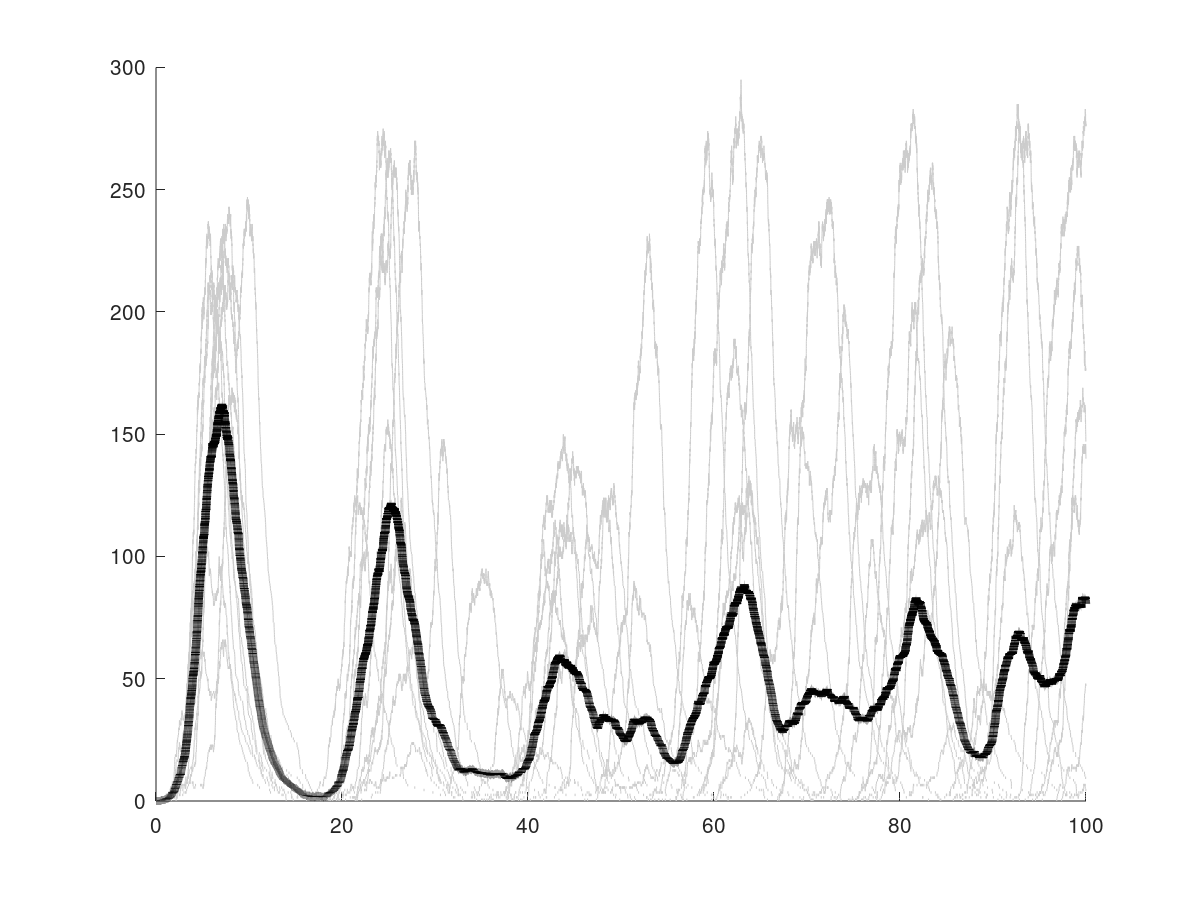
\includegraphics[width=\linewidth]{p1.png}
    \endminipage\hfill
    \minipage{0.33\textwidth}
      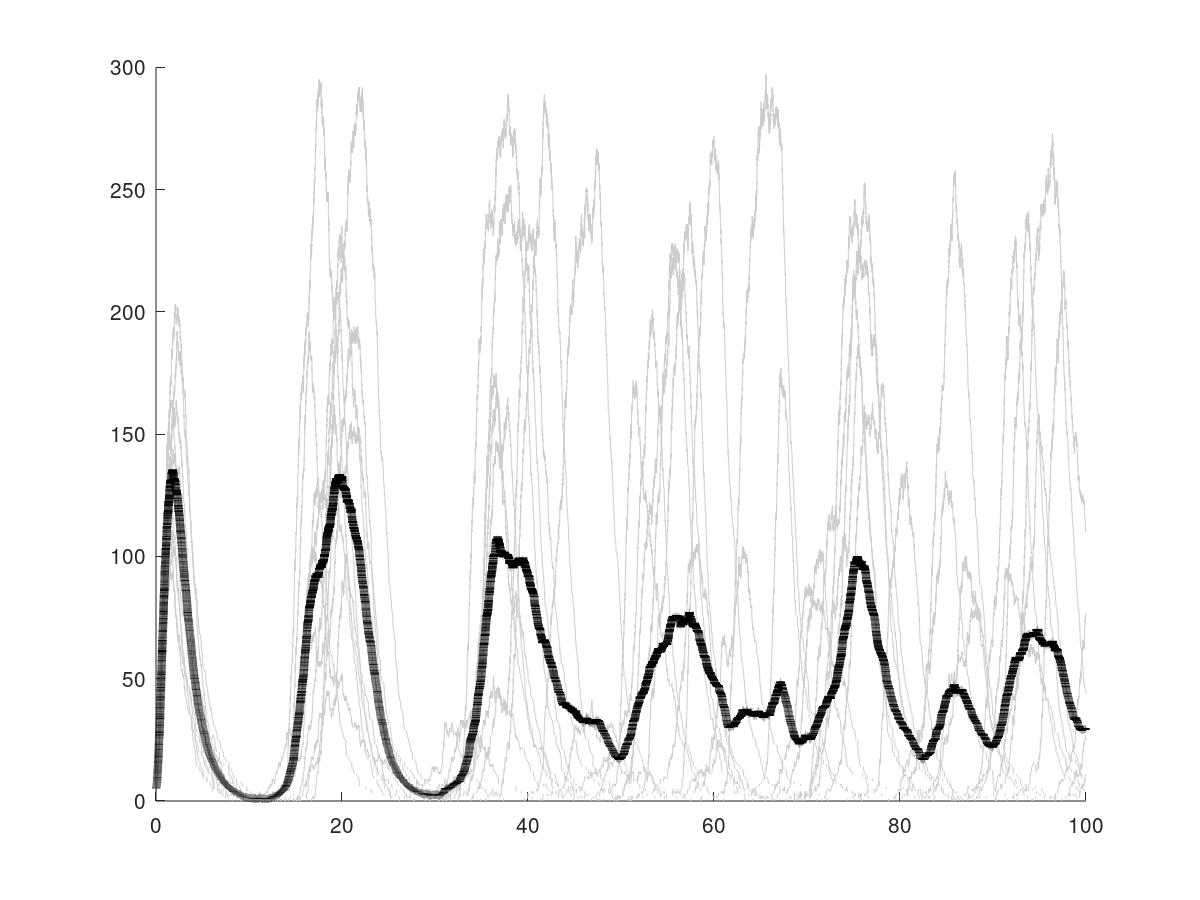
\includegraphics[width=\linewidth]{p2.png}
    \endminipage\hfill
    \minipage{0.33\textwidth}%
      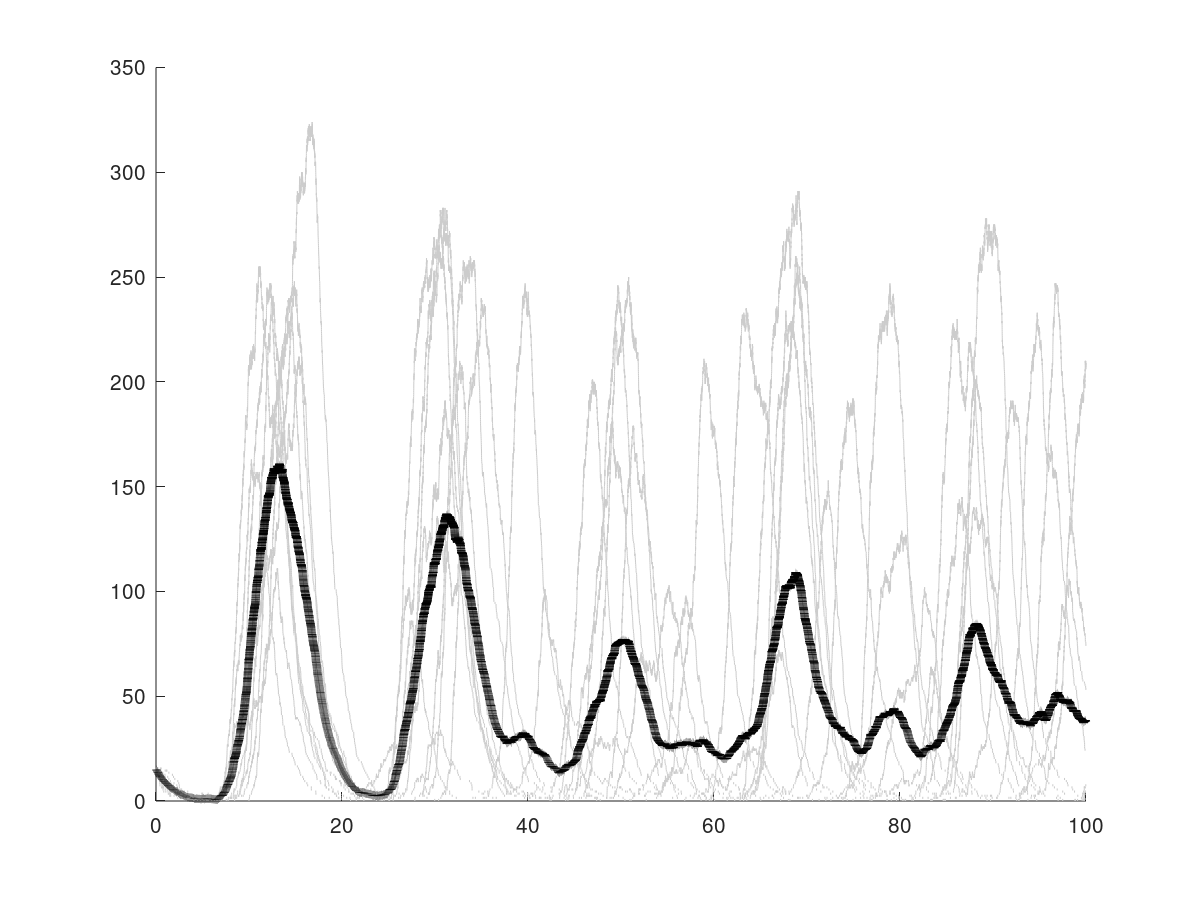
\includegraphics[width=\linewidth]{p3.png}
    \endminipage
    \caption{Multiple simulations of the Repressilator gro model. From left to right: p1, p2, p3. Black lines are used to indicate an average simulation, whilst the various grey lines are used to indicate the concentration of the respective protein at each individual simulation.}
    \label{fig:tons_of_simulations}
    \end{figure}

\subsection{Compiled SBML Simulation and Comparison}

    This section presents the results of a simulation of the compiled SBML document on Copasi, along with a comparison between it and a simulation of the original ODEs (1) in Octave. The Copasi simulation is presented on the left part of Figure~\ref{fig:repressilator_comparison} and the Octave one to the right.
    
    \begin{figure}[ht]
    \centering
    \minipage{0.5\textwidth}
      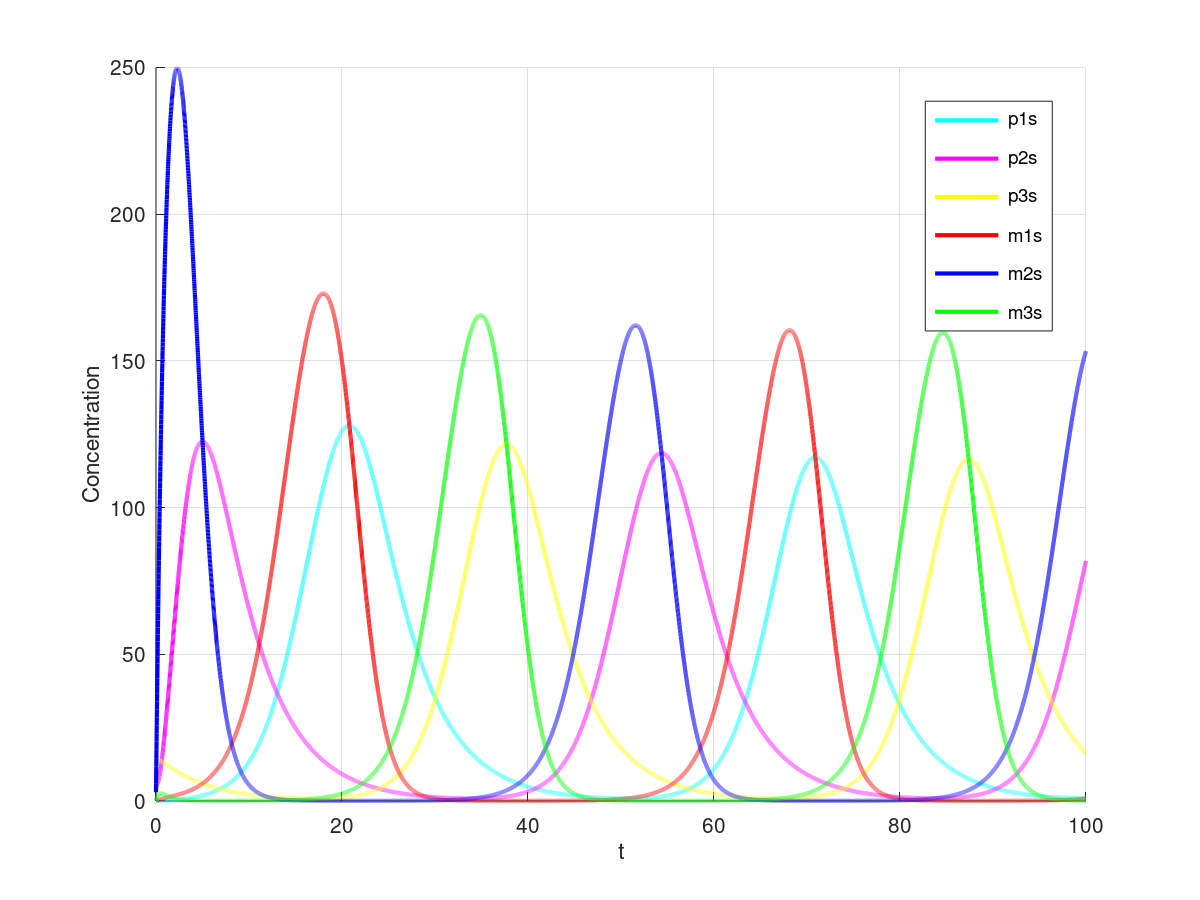
\includegraphics[width=\linewidth]{repressilator_octave.png}
    \endminipage\hfill
    \minipage{0.5\textwidth}
      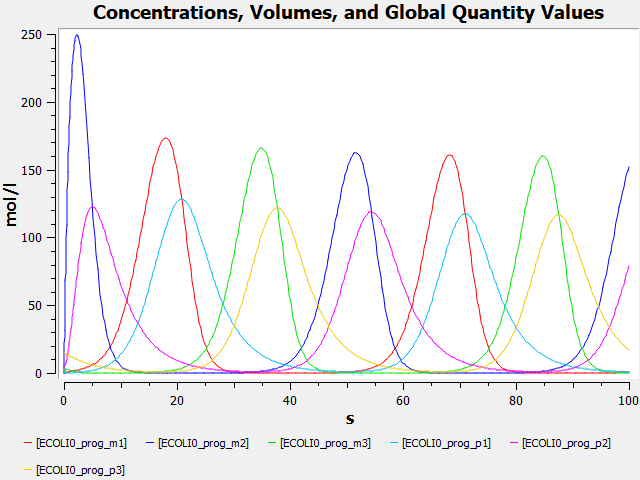
\includegraphics[width=\linewidth]{repressilator_copasi.png}
    \endminipage\hfill
    \caption{Comparison between the Octave model and compiled gro model for the Repressilator.}
    \label{fig:repressilator_comparison}
    \end{figure}

    As depicted at Figure~\ref{fig:repressilator_comparison}, both simulations yielded the same values on concentration over the simulation's duration. Such results demonstrate the effectiveness of the proposed compilation scheme, which besides reducing the coding effort for biological devices, grants a successful simulation of the generated SBML model.

 
\section{Conclusion \& Future Works}


    This paper presented a compilation scheme to the design and specification of biological devices using a framework that abstracts low level SBML constructs with higher level ones found in the gro programming language. The framework combines a code translator and Tellurium to map gro files to SBML documents. The proposed framework along with the gro mappings were illustrated through the compilation of a gro model for the Repressilator into an equivalent SBML document. They were also evaluated based on the comparison of two simulations: on for the resulting model and another for the original model (1).

    As future work, we intend to address the set of unrecognized gro language features. In particular, we plan to incorporate signals into our framework, enabling cell to cell communication. We also want to annotate the generated SBML document in cases where the source code contains features not recognized by our framework. This should, at the very least, notify tools which use our framework that some part of the source code was not translated into the SBML document and in other cases help the tool figure out how to deal with the syntactical mismatch.


% references
\bibliographystyle{sbc}
\bibliography{sbc-template}
\end{document}